\section{Requirements}
\label{requirements}

\begin{figure}[h]
\centering
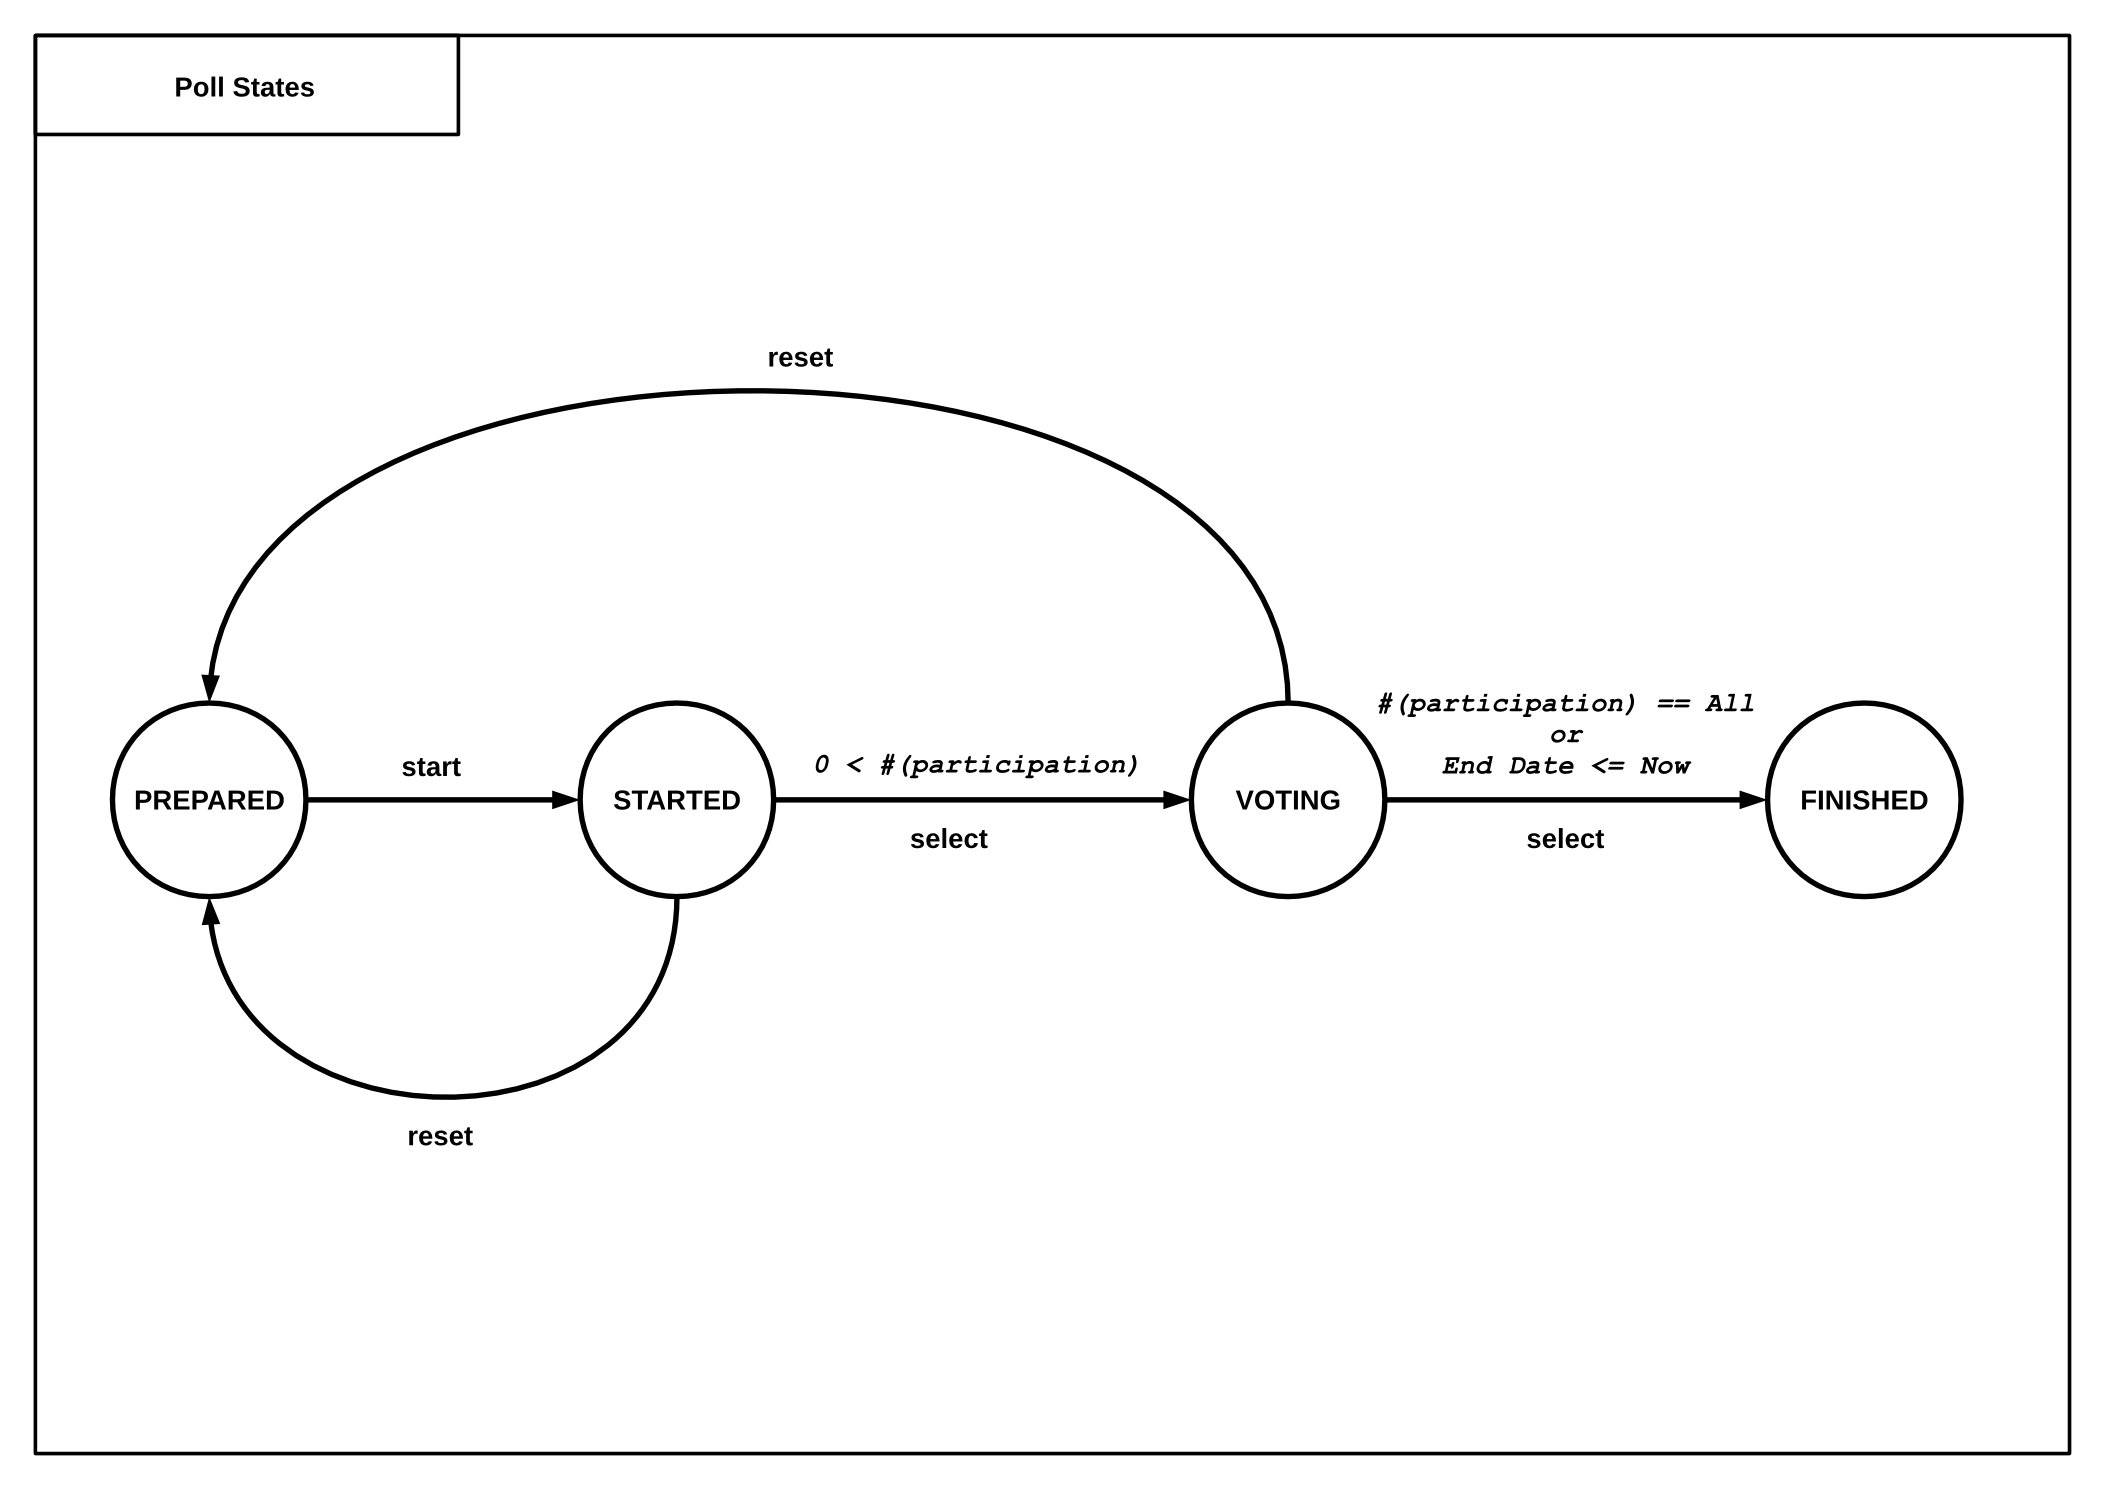
\includegraphics[width=0.9\textwidth]{png/poll-states.png}
\caption{Poll States}
\end{figure}

In this section the requirements realised by the system are listed. The enumeration mirrors the requirement list defined in \cite{Votes14}. The identifications numbers are identical. Requirements that are not completely implemented are left out.

% TODO: remove MANDATORY... and add if realized. Maybe with short description.

\subsection{Functional Requirements}
  \begin{itemize}
\item Polls


1.1. The system must support electronic polls with one or more items. MANDATORY


1.2. Each poll must have a title. The title has to be unique (scope is system). MANDATORY


1.3. Each poll must have a description. MANDATORY


1.4. Each poll must have a voting period (start and end date with time). MANDATORY


1.5. Each poll must have at least one item. MANDATORY


1.6. The system must allow to group arbitrary many items into one poll. MANDATORY


\item Poll states


2.1. The system must implement poll states. Polls be in one of four states: PREPARED, STARTED,
VOTING, FINISHED. State changes are specified in figure XXX. MANDATORY


2.2. When all participants submitted their votes, the system must set the poll to FINISHED.
MANDATORY


2.3. An organizer must be able to extend the voting period when a poll is in state STARTED or
VOTING. OPTIONAL


\item Organizers


3.1. The system must allow all university members to act as organizers. MANDATORY


3.2. Organizers must identify themselves with username and password. MANDATORY


3.2.1.University members can be identified by the LDAP service provided by the GHRKO
computing center. OPTIONAL


3.2.2.If LDAP is not used, an administrator must be able to create organizer accounts. OPTIONAL


3.3. An organizer must be able to conduct arbitrary many polls. MANDATORY


3.4. The system shall provide a preview mode that allows organizers to view how their polls look
like when a participant fills in her choices. OPTIONAL


3.5. The system can provide a possibility to add further organizers to a poll. Each organizer must
have the same options. OPTIONAL


3.5.1.An organizer must be able to change the organizer list.


3.5.2.An organizer must not be able to remove herself from the organizer list.


\item Administrators


4.1. The system must support an administrator role. OPTIONAL


4.2. Administrators must have the ability to delete polls (including all votes) from the system. OPTIONAL


4.3. Administrators must not be able to view votes nor results of polls which they didn’t organize.
OPTIONAL


4.4. Administrators must be able to create and delete user accounts, if no LDAP authentication is
provided (see requirement XXX). OPTIONAL


\item Participants


5.1. The organizer of a poll must be able to invite 3 to arbitrary many participants. In polls with
less than 3 participants, anonymity can not be asserted. MANDATORY


5.2. Each participant must be identified by her email address. MANDATORY


5.3. The system shall support participants from outside the university. OPTIONAL


5.4. After a poll is STARTED by the organizer, each participant must be informed via email about
the poll. OPTIONAL (University mail server must not be „mis-used“, it’s sufficient to display
the mail content on a web page)


5.5. The information mail must include the title of the poll, the start and end dates, the number of
participants, and a token. MANDATORY


5.6. The information can also contain a hyperlink immediately referring to the voting page with a
pre-filled token field. OPTIONAL


\item Participant lists


6.1. The organizer must be able to modify the participant list until a poll is STARTED. MANDATORY


6.2. The system can provide a means to comfortably create participant lists, e.g. by pasting
email addresses from other applications such as spread sheets or KLIPS. OPTIONAL


6.3. The system shall provide a means to store participant lists for easy reuse in subsequent
polls. OPTIONAL


6.3.1.The stored participant lists must be private to each organizer.


6.3.2.Each stored participant list must have a unique name (scope is per organizer).


\item Tokens


7.1. The token must be randomly chosen. MANDATORY


7.2. The token must be unique (scope is system). MANDATORY


7.3. The token must be long enough to make it very very improbable that anybody can forge a
valid token. MANDATORY


\item Anonymity


8.1. The system must ensure anonymity. MANDATORY (with reasonable effort)


8.2. At any point in time it must be impossible to identify which participant submitted which vote.
This also must to be guaranteed for polls with participation tracking. MANDATORY


8.3. The system must ensure that a token can not be associated with a vote. MANDATORY


\item Participation tracking


9.1. The system must provide an option to enable participation tracking for a poll. OPTIONAL


9.2. The system can provide an option to configure automatic reminders via E-Mail. OPTIONAL


\item Submitting a vote


10.1.The system must provide a web page to submit a vote. MANDATORY


10.2.The voting page must present an input field for a participant’s token. MANDATORY


10.3.The token input field can be pre-filled (see requirement XX). OPTIONAL


10.4.After the token was verified, the system must display the items. MANDATORY


10.5.The system must present a button to submit a vote. MANDATORY


10.6.After a vote was submitted, the token used for that vote must be invalidated (i.e. it can’t be
re-used, participants can not change their vote after submitting). MANDATORY


10.7.The system must allow to cancel a voting (e.g. by closing the browser, or by clicking a cancel
button). MANDATORY


10.8.The token used in cancelled voting must be re-useable later. MANDATORY


10.9.For a cancelled voting, the system must not remember any of the choices. OPTIONAL


10.10.The system shall ensure that subsequent participants using the same browser window
can not restore the previous choice (e.g. by the „go back“ function or by auto fill capabilities
of browsers). OPTIONAL


\item Abstain from voting


11.1.The system must provide a means to abstain from voting (Enthaltung oder ungültige
Stimme) for each item of a poll. MANDATORY


11.2.The system can provide a means to abstain from voting for a complete poll (this is equivalent
to abstaining from all items). OPTIONAL


\item Types of items


12.1.The system must support different types of items. MANDATORY


12.2.The items of a poll must have a title (titles have to be unique with scope poll). MANDATORY


12.3.The options of an item must have a short name and a description. MANDATORY


12.4.The system must support YES/NO items. In this case, the short names of the options are
„yes“ and „no“. MANDATORY


12.5.The system must support 1 OF N items. Participants can choose exactly one of zwo or
more options. MANDATORY


12.6.The system must support M OF N items. Participants can choose at most M of two or
more options (M $\leq$ N). OPTIONAL


12.7.The system can support 1 OF N items with a free text option. Participants can choose one
of the predefined options. Alternatively, they can enter a free text to indicate their choice.
OPTIONAL


12.8.The system can support M OF N items with up to M free text options. Participants can
choose at most M of the predefined options. Alternatively, they can can use less than M
predefined options an enter the rest of their choices into free text fields. OPTIONAL


\item Results


13.1.An organizer must be able to view the results of a poll after the voting period is FINISHED.
MANDATORY


13.2.Nobody must be able to view (intermediate) results in the STARTED and VOTING states.
MANDATORY

\end{itemize}

subsection{Non-Functional Requirements}
